\subsection{Architekturdiagramm }

Im dritten Kapitel wurden alle benötigten Dienste ausgewählt und ihre Notwendigkeit erläutert.
Nun muss aus allen Komponenten eine zusammenhängende Architektur aufgebaut werden.
Das folgende Diagramm soll die Verbindung zwischen allen Diensten aufzeigen:

\begin{figure}[htbp]
    \centering
    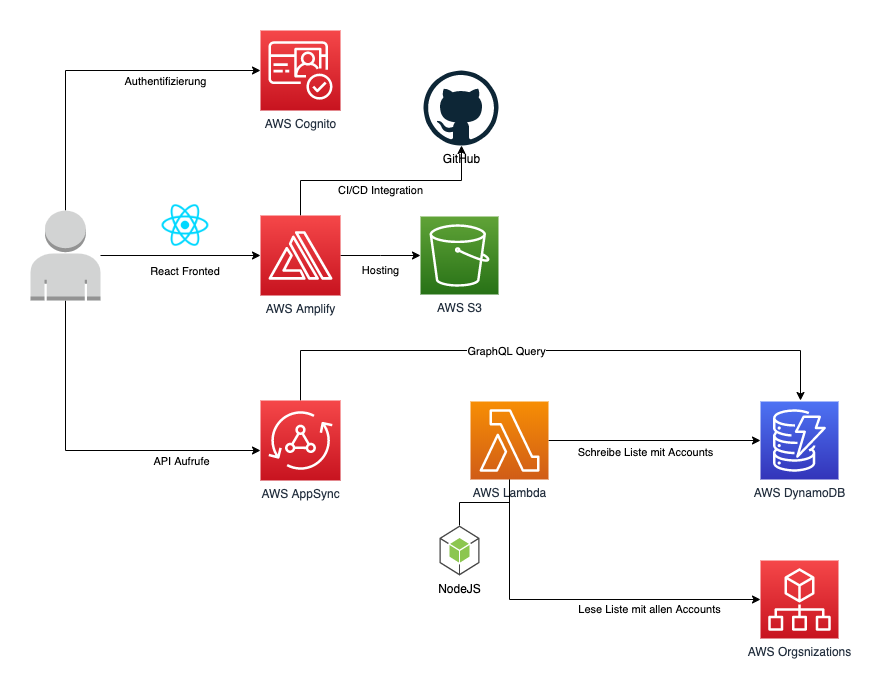
\includegraphics[width=1.0\textwidth]{50-Implementierung/Architektur.png}
    \caption{Übersicht der Architektur}
    \label{fig:meine-grafik}
\end{figure}

Das Diagramm zeigt die Kommunikationswege zwischen allen Diensten.
Sobald Anwender die Webanwendung aufrufen, kommunizieren sie mit den Diensten Cognito, Amplify Hosting sowie AppSync.
AppSync und das React-Frontend wiederrum greifen auf die DynamoDB-Tabelle zu, um die benötigten Daten abzufragen.
Die Lambda-Funktion sorgt im Hintergrund dafür, dass die Daten in der Tabelle stets aktuell sind.

Die Umsetzung der Anwendung erfolgt in fünf einzelnen Schritten.
Erzeugt werden alle Dienste über die Amplify CLI.
Zuerst müssen alle Voraussetzungen erfüllt werden und sowohl ein React-Projekt als auch Amplify initialisiert werden.
Zu den Voraussetzungen zählt das Installieren aller benötigten Pakete und der Zugang zu einem AWS Account.
Im zweiten Schritt wird die GraphQL API über die Amplify CLI bereitgestellt, welche automatisch die benötigten DynamoDB-Tabellen erzeugt.
Während des dritten Schritts wird die Lambda-Funktion erstellt, welche die Backend-Logik zur Verfügung stellt.
Der vierte Schritt hat das Ziel eine Authentifizierung mit Cognito bereitzustellen.
Zum Testen wird eine lokale Umgebung verwendet, sodass der Code erst nach Fertigstellung hochgeladen wird und die Anwendung zuvor nicht aufgerufen werden kann.
Das erlaubt ein schnelleres Testen und die Sicherheit, dass keine Daten öffentlich zugänglich sind.
Zuletzt kann die lokale Anwendung, sofern sie ordnungsgemäß funktioniert, bei AWS gehosted werden, sodass sie über das Internet zugänglich ist.

In den folgenden Abschnitten werden alle einzelnen Schritte im Detail erläutert sowie auf potenzielle Probleme bei der Umsetzung hingewiesen.

\subsection{AWS Accountstruktur }

Zuerst ist es notwendig die Struktur der AWS Accounts innerhalb der Mediengruppe RTL zu verstehen.
Zum einem ist es notwendig, da entschieden werden muss in welchem AWS Account die Webanwendung umgesetzt wird.
Zum anderen benötigt die Lambda-Funktion ebenfalls Zugriff auf den Dienst AWS Organizations.

Wie bereits in der Einleitung erwähnt besitzt die Mediengruppe RTL über 150 AWS Accounts.
Dabei werden pro Entwicklungsumgebung und pro Funktion bzw. Projekt einzelne Accounts erstellt.
Aus Sicherheitsgründen wird dementsprechend immer eine separate Produktiv- und eine oder mehrere, Testumgebungen erzeugt.
Dadurch kann der Zugriff auf jeweilige Umgebungen eingeschränkt werden.
Zudem ist eine bessere Kostenzuweisung durch Trennung möglich.
Beispiele für solche Accounts sind etwa \verb+Ntv-Streaming-Dev+ oder \verb+Ntv-Web-Prod+.
Jeder der Accounts ist grundsätzlich unabhängig und weißt nur über die gemeinsame Organization eine Verbindung auf.
In dem Beispiel Ntv wird zum Beispiel zwischen der Streaming Plattform und dem Frontend unterschieden.
Zusätzlich existieren jeweils eine \verb+Dev+ und eine \verb+Prod+ Umgebung.
Daneben ist es möglich, dass noch weitere Accounts oder Entwicklungen benötigt werden, etwa eine \verb+PreProd+ Umgebung.

Wie bereits im Abschnitt \ref{LambdaEntscheidung} \nameref{LambdaEntscheidung} erwähnt, werden alle Accounts zentral über den Dienst AWS Organizations erstellt.
Es wird Zugriff auf den Master-Account benötigt um Informationen zu allen Accounts zu erhalten.

Für die Abteilung Datacenter and Clouds gibt wurden speziell zum Testen und Probieren Accounts erstellt.
Der Account \verb+Cbc-Clouds-Sandbox+ eignet sich für eine erste Testumgebung daher optimal.
Wird die Anwendung in Zukunft produktiv genutzt, kann sie ohne viel Aufwand in einen anderen Account migriert werden.


\subsection{Amplify Voraussetzungen}

\subsubsection{Einrichtung Amplify CLI}
\label{EinrichtungAmplify}
Bevor mit der Amplify CLI gearbeitet werden kann, muss sichergestellt sein, dass alle benötigten Pakete installiert sind und ein Zugang zu einem AWS Account existiert.
Für die Verwendung von Amplify müssen die Pakete \verb+Node.js+ (Version \verb+>+ 10.x), \verb+npm+\footnote{Npm steht für Node Package Manager und ist ein Paketmanager für NodeJS. Mithilfe von npm können weitere Pakete installiert werden.} (Version \verb+>+ 5.x) und \verb+git+ (Version \verb+>+ 2.14.1) installiert werden.
Mithilfe von \verb+npm+ kann im Anschluss mit folgendem Befehl \verb+npm install -g @aws-amplify/cli+ die Amplify-CLI installiert werden.

Als nächstes benötigt die Amplify-CLI Zugang auf den AWS Account \verb+Cbc-Clouds-Sandbox+.
Hierfür muss ein AWS IAM User mit Credentials angelegt werden.
Diesen Prozess kann ebenfalls Amplify übernehmen.
Die Konfiguration wird mit dem Befehl \spverb+amplify configure+ gestartet.

\begin{verbatim}
    # amplify configure
    Follow these steps to set up access to your AWS account:

    Sign in to your AWS administrator account:
    https://console.aws.amazon.com/
    Press Enter to continue

    Specify the AWS Region
    ? region:  eu-central-1
    Specify the username of the new IAM user:
    ? user name:  amplify-kumo
    Complete the user creation using the AWS console
    https://console.aws.amazon.com/iam/home?region=undefined#/users$new?step=final&accessKey&userNames=amplify-kumo&permissionType=policies&policies=arn:aws:iam::aws:policy%2FAdministratorAccess

    Press Enter to continue

    Enter the access key of the newly created user:
    ? accessKeyId:  ********************
    ? secretAccessKey:  ************************

    Successfully set up the new user.
  \end{verbatim}

Es wird nach der gewünschten Region sowie Benutzernamen gefragt.
Anschließend öffnet sich ein neues Browserfenster und der Vorgang kann fortgesetzt werden.
In Browser bestätigt man das Erstellen des Benutzers und erteilt ihm Administratorberechtigungen.
Die im Browser angezeigten IAM Schlüssel werden in der CLI eingegeben und der Vorgang ist abgeschlossen.\cite[]{ImpVoraus}

Hinweis: Der interne Name des Projektes lautet Amplify-Kumo.
Kumo ist die japanische Bezeichnung für \glqq Cloud\grqq.


\subsubsection{Einrichtung React Projekt}

Bevor Amplify konfiguriert werden kann, muss ein React Projekt erstellt werden.
Dafür bieten die Entwickler von React den Befehl \verb+npx create-react-app+ an, welcher eine fertige Entwicklungsumgebung aufsetzt.
Dabei werden Aspekte wie die Ordnerstruktur, benötigte JavaScript-Pakete oder auch die Konfiguration eines Webservers übernommen.\cite[]{ReactNew}
Um das Projekt zu erstellen und im Anschluss den Webserver zu starten sind folgende Befehle notwendig:

\begin{verbatim}
npx create-react-app amplify-kumo
cd amplify-kumo
npm start
\end{verbatim}

Der Webserver ist unter der Adresse \verb+http://localhost:3000+ erreichbar und zeigt eine Testseite von React.


\subsubsection{Konfiguration Amplify}

Nachdem das React Projekt erfolgreich erstellt wurde, kann Amplify konfiguriert werden.
Im Anschluss ist es möglich alle gewünschten Dienste mit Amplify hinzuzufügen.

Zur Konfiguration muss \verb+amplify init+ ausgeführt werden.
Hinweis: Für eine bessere Übersicht ist die folgende Ausgabe gekürzt.

\begin{verbatim}
[143302S0:amplify-kumo] master # amplify init
  Enter a name for the project: amplifykumo
  Enter a name for the environment: dev
  Choose your default editor: Visual Studio Code
  Choose the type of app that you're building: javascript
Please tell us about your project
  What javascript framework are you using: react
  Source Directory Path:  src
  Distribution Directory Path: build
  Build Command:  npm run-script build
  Start Command: npm run-script start

Using default provider  awscloudformation
Do you want to use an AWS profile? (Y/n) Y
Please choose the profile you want to use: amplify-kumo
Initializing project in the cloud...

[...]

CREATE_COMPLETE DeploymentBucket AWS::S3::Bucket
CREATE_COMPLETE UnauthRole       AWS::IAM::Role
CREATE_COMPLETE AuthRole         AWS::IAM::Role
 Initializing project in the cloud...

CREATE_COMPLETE amplify-kumo AWS::CloudFormation::Stack
Successfully created initial AWS cloud resources for
deployments.
Initialized provider successfully.
Initialized your environment successfully.

Your project has been successfully initialized and
connected to the cloud!

\end{verbatim}

Als erstes werden allgemeine Informationen benötigt, wie der Projektname oder das gewünschte Javascript-Framework.
Die darauffolgenden Pfade und Befehle sind nicht geändert worden.
Des weiteren wird der, in \ref{EinrichtungAmplify} \nameref{EinrichtungAmplify} erstellte, IAM User angegeben.
Nach kurzer Zeit ist das Amplify Projekt bereits in der Cloud erstellt worden und verfügbar.

Wie im Code ersichtlich, benutzt Amplify den Dienst AWS Cloudformation, sodass die gesamte Konfiguration in einem Template festgehalten wird.
Mit AWS CloudFormation ist möglich Templates zur Modellierung und Bereitstellung von AWS-Ressourcen zu erstellen.
Die Templates unterstützen JSON und YAML.
Amplify übersetzt alle Befehle in ein Cloudformation Template und startet es.
Da die gesamte Konfiguration der Cloudformation-Templates von Amplify übernommen wird, ist keine Bearbeitung erforderlich.

Außerdem wird bei der Initialisierung ein S3 Bucket sowie IAM-Rollen erstellt.
Das Bucket dient als Speicher für alle Konfigurationen und Templates.
Die IAM-Rollen werden für die Authentifizierung von Amplify benötigt.

Es wurden alle Voraussetzungen erfüllt und die einzelnen Dienste können dem Projekt hinzugefügt werden.
